\section{Enllaços hypermedia, la navegació entre recursos}

    \paragraph{}
    Com hem comentat en l’apartat anterior, els recursos emmagatzemen informació sobre les URI dels recursos relacionats. Aquestes URI són anomenades enllaços hypermedia i permeten la navegació  entre els diferents recursos del model de dades.

    Per posar un exemple, imaginem el recurs Persona. Aquest conté enllaços hypermedia que apunten als recursos que conformen el concepte Parella, Pares, Fills, Fonts d'informació, Ascendència, Descendència i Memòries. Cada un d'aquests recursos apuntats conté informació específica i d'interès respecte a la persona consultada.

    La figura~\ref{fig:hypermedia} reflecteix com el recurs Persona és accessible a través de l'Arbre Familiar de FamilySearch i com les diferents relacions i recursos, associats a una persona, són connectats a través dels enllaços hypermedia d'aquest.

    \begin{figure}[h]
        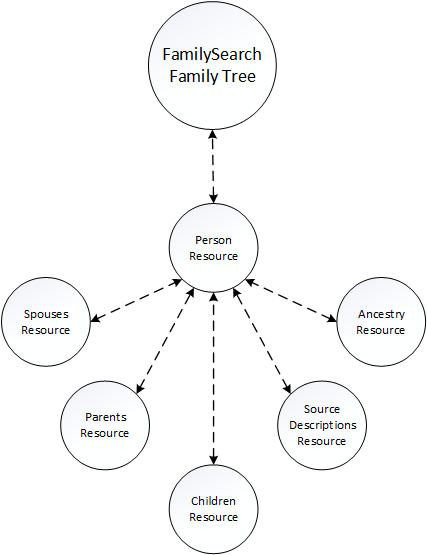
\includegraphics[scale=0.8]{05/01_hypermedia}
        \centering
        \caption{Enllaços hypermedia del recurs Persona.}\label{fig:hypermedia}
    \end{figure}

    Volem aprofitar aquest apartat de la memòria per recordar, que en el moment en què la nova versió del back-end, Family Tree, es trobi desplegada per complet a producció, el recurs Persona no contindrà més els enllaços hypermedia a tots aquests recursos, sinó que les relacions de parella o paternals, es trobaran incloses dins del mateix recurs Persona.

    De totes maneres, el concepte dels enllaços hypermedia seguirà sent vàlid de cara a les relacions del recurs Persona amb la resta de recursos vinculats i per tota la resta de relacions entre els diferents recursos de l'API de FamilySearch.

    Els enllaços hypermedia cobren especial interès a l'hora de crear aplicacions robustes que es vegin el menys afectades possible per canvis en la localització o crida dels recursos.

    El primer gran avantatge d’utilitzar aquests enllaços és que no cal implementar en el codi, de forma específica, les URI d'accés a cada recurs. D'aquesta forma, s'aconsegueix evitar que en cas de canvis en les URI, sigui necessari realitzar modificacions en el codi de les nostres aplicacions.

    El segon, és que si es coneix un sol punt d’entrada al sistema, les aplicacions ja no requeriran més informació per tal de navegar entre els diferents recursos de la resposta. D'aquesta forma, podríem descriure els enllaços hypermedia com una espècie d'índexs que permeten explorar i navegar a través del conjunt de recursos que conformen les respostes de l'API de FamilySearch. 
